We isolate connectivity in a supervised task with exact action values.
Training uses 40,000 independent uniform nine-node geometries, each with two
forests obtained from different matchings of three prescribed heads to three
prescribed tails; the remaining three vertices are singletons, including the
selected source. Validation has 3,000 different geometries. Each test condition
has 4,500 new geometries from three data seeds. Both members of a pair always
remain in the same split. Zero-shot tests vary the node count to 7, 11, and 13
or replace uniform coordinates by three Gaussian clusters.

Blind and aware predictors use the same three-layer, width-128 Transformer
(415,489 parameters), with no positional encoding, and 10,000 AdamW updates
of batch 512. Both receive coordinates relative to the source, head/tail
roles, and singleton/non-singleton indicators. This enriched blind observation
is deliberately more informative than the audited host interface. Only the
aware predictor receives true partner-coordinate displacements. Models
regress exact action regrets; validation regret selects the checkpoint.
Three independent initialization seeds share the data and minibatch streams.
An additional control trains the same network with independent random
pairings, preserving active feature channels without providing true connectivity.

\begin{table}[t]
\centering\small
\begin{tabular}{lrrrrr}
\toprule
Test & Blind & Random pairing & True pairing & Assignment & Nearest \\
\midrule
Uniform 9 & 0.03422 & 0.03374 & 0.00645 & 0.03629 & 0.07744 \\
Clustered 9 & 0.01726 & 0.01778 & 0.00649 & 0.01667 & 0.03354 \\
Uniform 7 & 0.03338 & 0.03502 & 0.00693 & 0.04154 & 0.08148 \\
Uniform 11 & 0.03392 & 0.03389 & 0.01227 & 0.03045 & 0.07081 \\
Uniform 13 & 0.03332 & 0.03295 & 0.01887 & 0.02626 & 0.06704 \\
\bottomrule
\end{tabular}

\caption{Exact fixed-source completion regret, averaged over three training
seeds and paired states. This is not complete-tour solver performance.
The random-pairing control and assignment-relaxation heuristic are supplementary
controls designed after pilot validation. All final selection uses validation.
Every condition has 4,500 independent test geometries.}
\label{tab:conditional}
\end{table}

The true-pairing predictor reduces IID regret from 0.03422 to 0.00645
(81.2\%). The paired absolute reduction is 0.02777, with a geometry-and-seed
bootstrap 95\% interval [0.02572, 0.02981]. The independently trained random-pairing
control obtains 0.03374, close to the blind predictor. Thus active extra input
channels alone do not explain the benefit. Table~\ref{tab:conditional} retains
distribution and size shifts and inexpensive nearest-head and cycle-cover
assignment comparators. The assignment score uses a lower-bound relaxation;
it is not an exact-completion oracle.

\begin{figure}[t]
\centering
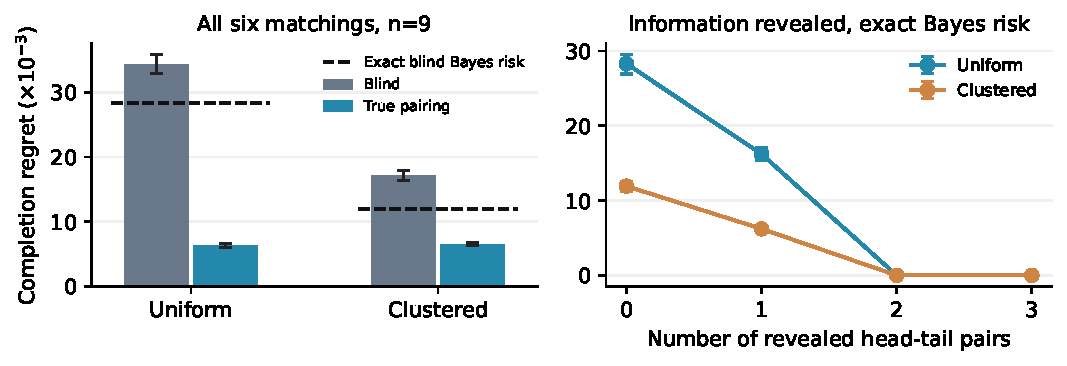
\includegraphics[width=\linewidth]{figures/conditional.pdf}
\caption{A supplementary exhaustive observation-class evaluation on the same
held-out geometries. Left: all $3!=6$ possible matchings, with learned-model
means over three seeds and geometry-bootstrap intervals. Right: reveal the
partners of a predetermined subset of heads and recompute exact Bayes risk.
These curves concern the specified observation family, not native-host occupancy.}
\label{fig:conditional}
\end{figure}

Enumerating all six matchings instead of a sampled pair yields an exact
Bayes risk of 0.02831 for the enriched blind observation on uniform geometries.
The aware model achieves 0.00633 on this same family
(Figure~\ref{fig:conditional}). Revealing one prescribed partner reduces
the risk to 0.01622; revealing two determines the third and reduces it to zero.
This full-family computation avoids confusing a pair-aware oracle with the
Bayes limit for the actual controlled observation.

Swapping the two true associations at test time while keeping model weights
fixed raises IID regret to 0.06271. This is a sensitivity intervention and a
distribution change, not a retrained baseline. Together with the independently
trained random-pairing control, it supports the role of connectivity in the
conditional task. Independent Held--Karp checks of stored labels agree with
enumeration to floating-point precision; coordinate hashes exclude leakage,
blind predictions are exactly identical within each pair, and the largest
measured permutation-equivariance error is $2.98\times10^{-7}$.
